% !TeX spellcheck = en_GB
%%%%%%%%%%%%%%%%%%%%%%%%%%%%%%%%%%%%%%%%%%
%                                        %
%    Engineer thesis LaTeX template      % 
%                                        %
%%%%%%%%%%%%%%%%%%%%%%%%%%%%%%%%%%%%%%%%%%



\documentclass[a4paper,twoside,12pt]{book}
\usepackage[utf8]{inputenc}                                      
\usepackage[T1]{fontenc}  
\usepackage{amsmath,amsfonts,amssymb,amsthm}
\usepackage[polish,british]{babel} 
\usepackage{indentfirst}
\usepackage{lmodern}
\usepackage{graphicx} 
\usepackage{hyperref}
\usepackage{booktabs}
\usepackage{tikz}
\usepackage{pgfplots}
\usepackage{mathtools}
\usepackage{geometry}
\usepackage[page]{appendix} 

\usepackage{setspace}
\onehalfspacing


\frenchspacing

\usepackage{listings}
\lstset{
	language={},
	basicstyle=\ttfamily,
	keywordstyle=\lst@ifdisplaystyle\color{blue}\fi,
	commentstyle=\color{gray}
}

%%%%%%%%%

 

%%%%%%%%%%%% FANCY HEADERS %%%%%%%%%%%%%%%

\usepackage{fancyhdr}
\pagestyle{fancy}
\fancyhf{}
\fancyhead[LO]{\nouppercase{\it\rightmark}}
\fancyhead[RE]{\nouppercase{\it\leftmark}}
\fancyhead[LE,RO]{\it\thepage}


\fancypagestyle{onlyPageNumbers}{%
   \fancyhf{} 
   \fancyhead[LE,RO]{\it\thepage}
}

\fancypagestyle{PageNumbersChapterTitles}{%
   \fancyhf{} 
   \fancyhead[LO]{\nouppercase{\it\rightmark}}
   \fancyhead[RE]{\nouppercase{\it\leftmark}}
   \fancyhead[LE,RO]{\it\thepage}
}


%%%%%%%%%%%%%%%%%%%%%%%%%%%
% listings 
\usepackage{listings}
\lstset{%
language=C++,%
commentstyle=\textit,%
identifierstyle=\textsf,%
keywordstyle=\sffamily\bfseries, %\texttt, %
%captionpos=b,%
tabsize=3,%
frame=lines,%
numbers=left,%
numberstyle=\tiny,%
numbersep=5pt,%
breaklines=true,%
morekeywords={descriptor_gaussian,descriptor,partition,fcm_possibilistic,dataset,my_exception,exception,std,vector},%
escapeinside={@*}{*@},%
%texcl=true, % wylacza tryb verbatim w komentarzach jednolinijkowych
}
%%%%%%%%%%%%%%%%%%%%%%%%%%%%%%%%%%%%

%%%% TODO LIST GENERATOR %%%%%%%%%

\usepackage{color}
\definecolor{brickred}      {cmyk}{0   , 0.89, 0.94, 0.28}

\makeatletter \newcommand \kslistofremarks{\section*{Remarks} \@starttoc{rks}}
  \newcommand\l@uwagas[2]
    {\par\noindent \textbf{#2:} %\parbox{10cm}
{#1}\par} \makeatother


\newcommand{\ksremark}[1]{%
{%\marginpar{\textdbend}
{\color{brickred}{[\foreignlanguage{polish}{#1}]}}}%
\addcontentsline{rks}{uwagas}{\protect{\foreignlanguage{polish}{#1}}}%
}

%%%%%%%%%%%%%% END OF TODO LIST GENERATOR %%%%%%%%%%% 

% some issues...

\newcounter{PagesWithoutNumbers}

\newcommand{\hcancel}[1]{%
    \tikz[baseline=(tocancel.base)]{
        \node[inner sep=0pt,outer sep=0pt] (tocancel) {#1};
        \draw[red] (tocancel.south west) -- (tocancel.north east);
    }%
}%

\newcommand{\MonthName}{%
  \ifcase\the\month
  \or January% 1
  \or February% 2
  \or March% 3
  \or April% 4
  \or May% 5
  \or June% 6
  \or July% 7
  \or August% 8
  \or September% 9
  \or October% 10
  \or November% 11
  \or December% 12
  \fi}


%%%%%%%%%%%%%%%%%%%%%%%%%%%%%%%%%%%%%%%%%%%%%%
% Helvetica font macros for the title page:
\newcommand{\headerfont}{\fontfamily{phv}\fontsize{18}{18}\bfseries\scshape\selectfont}
\newcommand{\titlefont}{\fontfamily{phv}\fontsize{18}{18}\selectfont}
\newcommand{\otherfont}{\fontfamily{phv}\fontsize{14}{14}\selectfont}

%%%%%%%%%%%%%%%%%%%%%%%%%%%%%%%%%%%%%%%%%%%%%%
%%%%%%%%%%%%%%%%%%%%%%%%%%%%%%%%%%%%%%%%%%%%%%
%%%%%%%%%%%%%%%%%%%%%%%%%%%%%%%%%%%%%%%%%%%%%%
%%%%%%%%%%%%%%%%%%%%%%%%%%%%%%%%%%%%%%%%%%%%%%
%%%%%%%%%%%%%%%%%%%%%%%%%%%%%%%%%%%%%%%%%%%%%%
%%%%%%%%%%%%%%%%%%%%%%%%%%%%%%%%%%%%%%%%%%%%%%
%%%%%%%%%%%%%%%%%%%%%%%%%%%%%%%%%%%%%%%%%%%%%%


\newcommand{\Author}{Wojciech Drzewiecki}
\newcommand{\Supervisor}{Krzysztof Simiński, PhD DSc}
\newcommand{\Consultant}{Name Surname, PhD}
\newcommand{\Title}{Central online voting system}
\newcommand{\Polsl}{Silesian University of Technology}
\newcommand{\Faculty}{Faculty of Automatic Control, Electronics, and Computer Science}



\begin{document} 
\kslistofremarks
\cleardoublepage
	
%%%%%%%%%%%%%%%%%%  Title page %%%%%%%%%%%%%%%%%%% 
\pagestyle{empty}
{
	\newgeometry{top=2.5cm,%
	             bottom=2.5cm,%
	             left=3cm,
	             right=2.5cm}
	\sffamily
	\rule{0cm}{0cm}
	
	\begin{center}
	
\includegraphics[width=29mm]{polsl}
	\end{center} 
	\vspace{1cm}
	\begin{center}
	\headerfont \Polsl
	\end{center}
	\begin{center}
	\headerfont \Faculty
	\end{center}
	\vfill
	\begin{center}
	\titlefont Engineer thesis
	\end{center}
	\vfill
	
	\begin{center}
	\otherfont \Title\par
	\end{center}
	
	\vfill
	
	\vfill
	 
	\noindent\vbox
	{
		\hbox{\otherfont author: \Author}
		\vspace{12pt}
		\hbox{\otherfont supervisor: \Supervisor}
		% \vspace{12pt}
		% \hbox{\otherfont consultant: \Consultant}
	}
	\vfill 
 
   \begin{center}
   \otherfont Gliwice,  \MonthName\ \the\year
   \end{center}	
	\restoregeometry
}
  

\cleardoublepage
 

\rmfamily
\normalfont


%%%%%%%%%%%% statements required by law and Dean's office %%%%%%%%%%
\cleardoublepage

\begin{flushright}
załącznik nr 2 do zarz. nr 97/08/09 
\end{flushright}

\vfill  

\begin{center}
\Large\bfseries Oświadczenie
\end{center}

\vfill

\foreignlanguage{polish}{Wyrażam  zgodę / Nie wyrażam zgody*  na  udostępnienie  mojej  pracy  dyplomowej / rozprawy doktorskiej*.}

\vfill

Gliwice, dnia {\selectlanguage{polish}\today}

\vfill

\rule{0.5\textwidth}{0cm}\dotfill 

\rule{0.5\textwidth}{0cm}
\begin{minipage}{0.45\textwidth}
{\begin{center}(podpis)\end{center}}
\end{minipage} 

\vfill

\rule{0.5\textwidth}{0cm}\dotfill 

\rule{0.5\textwidth}{0cm}
\begin{minipage}{0.45\textwidth}
{\begin{center}\rule{0mm}{5mm}(poświadczenie wiarygodności podpisu przez Dziekanat)\end{center}}
\end{minipage}


\vfill

* podkreślić właściwe

 


%%%%%%%%%%%%%%%%%%%%%  
\cleardoublepage

\rule{1cm}{0cm}

\vfill  

\begin{center}
\Large\bfseries Oświadczenie promotora
\end{center}

\vfill

\foreignlanguage{polish}{Oświadczam, że praca „\Title” spełnia wymagania formalne pracy dyplomowej inżynierskiej.}

\vfill



\vfill

Gliwice, dnia {\selectlanguage{polish}\today}

\rule{0.5\textwidth}{0cm}\dotfill 

\rule{0.5\textwidth}{0cm}
\begin{minipage}{0.45\textwidth}
{\begin{center}(podpis promotora)\end{center}}
\end{minipage} 

\vfill
 
 

\cleardoublepage


%%%%%%%%%%%%%%%%%% Table of contents %%%%%%%%%%%%%%%%%%%%%%
\pagenumbering{Roman}
\pagestyle{onlyPageNumbers}
\tableofcontents

%%%%%%%%%%%%%%%%%%%%%%%%%%%%%%%%%%%%%%%%%%%%%%%%%%%%%
\setcounter{PagesWithoutNumbers}{\value{page}}
\mainmatter
\pagestyle{PageNumbersChapterTitles}

%%%%%%%%%%%%%% body of the thesis %%%%%%%%%%%%%%%%%


\chapter{Introduction}
  According to ``V-Dem Annual Democracy Report 2019'', prepared by the Department of Political Science, University of Gothenburg,
  ``Democracy is still the most common type of regime [in the world]'' \cite{bib:v-dem_report}.
  In the advanced stage of internet age that we are living in right now, it is weird, that almost all democratic countries carry out their elections in voting wards.
  As the society becomes more and more up to date with the latest technical innovations, there will be a point in the future, 
  when some kind of remote voting becomes the most used voting method across the globe.
  For now the only technology that is available to vast majority of developed countries and may be considered as help in elections is the internet. 

  Objective of this thesis is to focus on functionalities and features of voting system capable of delivering safe and easy to use online voting.
  The solution has three core features: individual online voting, ward protocol sending and calculating results of an election.
  Every functionality is accessible through web browser communicating with application server which is processing the requests.
  All necessary data is held in a database and fetched when necessary.
  That is the most common solution available to us at the moment.

  First chapter of this thesis is dedicated to problem analysis. I focus on an idea of the perfect online voting system and review similar existing solutions.
  In the next chapter I state functional requirements, nonfunctional requirements and few possible use cases of an online voting system. 
  I also describe tools used in the application and propose their alternatives.
  After that, I focus on external and internal specification of the application itself. 
  External specification includes back to back guidelines for the user of the application, while internal specification includes information about implementation and overview of the backend of the system.
  I finish the thesis with verification and validation of the application and short conclusion chapter.

\chapter{Online voting systems}

\section{Introduction}

	Ever since internet was introduced in our lives, online election voting was a contentious issue.

	First of all, online voting would be convenient---right now voting is associated with going to a nearby ward, waiting in a queue, 
	complicated procedure of receiving a ballot and filling a ballot.
	Moreover, waiting for results could be decreased---now we have to wait for all the votes to be counted, protocols sent to commissions,
	summed up, and determination of the winners. All this can take over few dozen hours.
	Online voting would decrease that time hugely, at the same time being much more precise than counting by a person.
	
	On the other hand, there is significant trust issue. There will always be a person which have access to data, 
	and with such access that person could change elections results in a matter of seconds.
	Following this lead, even if nobody has access to data, we will never be sure that vote we cast is not changed somewhere in the logic of the application.
	We can eliminate that by developing open source application, which can be verified that it does not change something in the logic.
	This approach would create many more problems, of which two are: firstly, open source application can be investigated by everyone, 
	and with given source it is much easier to find a hole in the logic from which we can benefit.
	Secondly, even if we see view of that open source application, we can never be sure that logic behind it is not swapped.
	
	You can see a pattern here---for every argument there is a counter argument, which generates another problems. 
	There is no right answer in this debate.

\section{Ideal voting system}

  So what would be features of the perfect voting system? Let's investigate it along with flow of online voting.

  Before election, system administrator has to enter committees and candidates data into a system, register them for polls predicted for certain date, which he has entered at the beginning.
  Although he could handle registering candidates to certain committees, he cannot handle scope of managing whole committee during election. 
  It is best if administrator granted some chosen user privileges to manage certain committee inside the system---let's call him committee administrator.
  It is useful for example in case of allocation seats via D'Hondt method---it is a committee itself that wants to decide on order in closed list, there should be no third party involved.
  
  First, in order to cast a vote through internet, a citizen would have to register. What online voting system wants to achieve for citizens is to be able to cast a vote without leaving home.
  It makes sense that citizens would register also through the internet---for example in case of some injury, if someone could go out of home, they could also vote in a ward. 
  It creates a problem---how do we know that person on the other side of the screen is who he says he is. 
  Solution is two step authentication process---citizen registers with citizen id (for example PESEL in Poland), he is sent a text message or an email,
  but also receives registered letter of registration, both with activation codes, that only together allows him to register properly. 
  Registered letter allows to verify citizen willing to vote through internet without need of leaving the house. 
  Because email can be generated without interference of any third party person, code sent this way secures citizen from someone taking advantage of code in letter.
  Those two ways combined secure citizens account from being taken advantage of.

  Let's say a citizen registered successfully. On election day, he should be able to vote on exactly the same polls as he would personally, in ward.
  Citizen should be able to cast a vote only once, and his vote should be detached from his account---in no way should anybody be able to tell which vote belongs to which citizen.
  Although registered for online voting, a citizen should still be able to vote personally in ward. 
  However, once he voted in any of two ways, the second one should be automatically and immediately blocked. This requires for the system to work also in wards.
  Once user votes online or receives a ballot from commission in a ward, he should be immediately blocked for second type of voting.

  Citizen easily and securely voted either through internet or personally. Now his journey ends, he can go back to living his life. 
  What's left to do is to calculate results of election. However, system also has to take into account all votes casted in wards.
  Results can be calculated if and only if all wards have entered their protocols into the system.
  To do so, a member of a commission should be assigned with access to send the protocol to the system---let's call him a ward administrator. 
  Once that member is a registered user, he should be able to be assigned as particular ward admin by the system administrator.
  Then, he should be able to file in the protocol, once the election is closed for voting.
  
  After closing the election and collecting protocols from all wards, results of the election can be calculated.
  This information can be public and delivered to public on the same site that they voted on, as well as on official government electoral commission website.

\section{Overview of similar solutions}

  \subsection{Electronic voting in Estonia}
    In Estonia, voting is based on electronic citizen ID. It is mandatory and sufficient national identity document, which allows for secure remote authentication.
    To cast a vote, an Estonian needs a computer connected to the internet and equipped with card reader.
    They can authenticate using digital certificate included in their citizen card, and cast a vote on the internet \cite{bib:internet_voting_estonia}.

    This solution is problematic for several reasons:
    \begin{itemize}
      \item It is impossible to be easily implemented in countries without electronic citizen ID. 
        Providing such documents for most of society of the country is a long time process, measured in years rather than months.
      \item A card reader capable of reading such a card is not a common device---a citizen has to go somewhere with a card reader, if he wants to cast a vote.
      \item Electronic citizen ID is not an intellectual knowledge like password or token. 
        It is a physical device that can be easily stolen---and of course blocked in some department---but it may be too late and someone may have already taken advantage from owning someone else's citizen ID.
    \end{itemize}

\chapter{Requirements and tools}
\label{chap:req&tools}
  \section{Functional requirements}
    To better understand scope of the project, we define functional requirements:
    \begin{itemize}
      \item A citizen of a country that holds an online election in the application should be able to register.
      \item The application should allow registered citizens to vote on candidates of their preference.
      \item A vote of a citizen should be taken into account when calculating results of an election.
      \item A citizen should be able to cast only one vote per election.
      \item A vote of a citizen should not be trackable---no person should be able to tell which citizen voted on which candidate.
      \item A person designated as a ward administrator---and only that person---should be able to send a ward protocol to the system.
      \item Protocols sent from wards should be taken into account when calculating results of an election.
      \item A person designated as a committee administrator---and only that person---should be able to enter a committee's closed list candidates order to the system.
      \item An administrator of the application should be able to perform steps that lead to creation of an election identical to one provided to him.
      \item An administrator should be able to trigger calculation of the results of an election.
      \item Election results should not be calculated with some of ward protocols missing.
      \item An administrator should be able to grant privileges of ward and committee administrators to designated people separately.
      \item An administrator should not be able to perform actions in replacement of  a ward or committee administrator.
    \end{itemize}
    
    \ksremark{Jak system zapewnia anonimowość głosowania?}

  \section{Nonfunctional requirements}
    After reviewing functional requirements, we can define nonfunctional requirements:
    \begin{itemize}
      \item User interface should be understandable to English speaking individuals.
      \item The application should be implemented in Java, with help of Spring Boot and related frameworks for the backend, 
      and Thymeleaf template engine for the frontend.
      \item The application should store all necessary data in a MySQL database.
      \item The application should hash all sensitive data stored in a database.
      \item The application should offer all available functionalities on Google Chrome version 79.
    \end{itemize}
  \pagebreak

  \section{Use cases}
    \subsection{Citizen use case UML}
    \begin{figure}[h]
      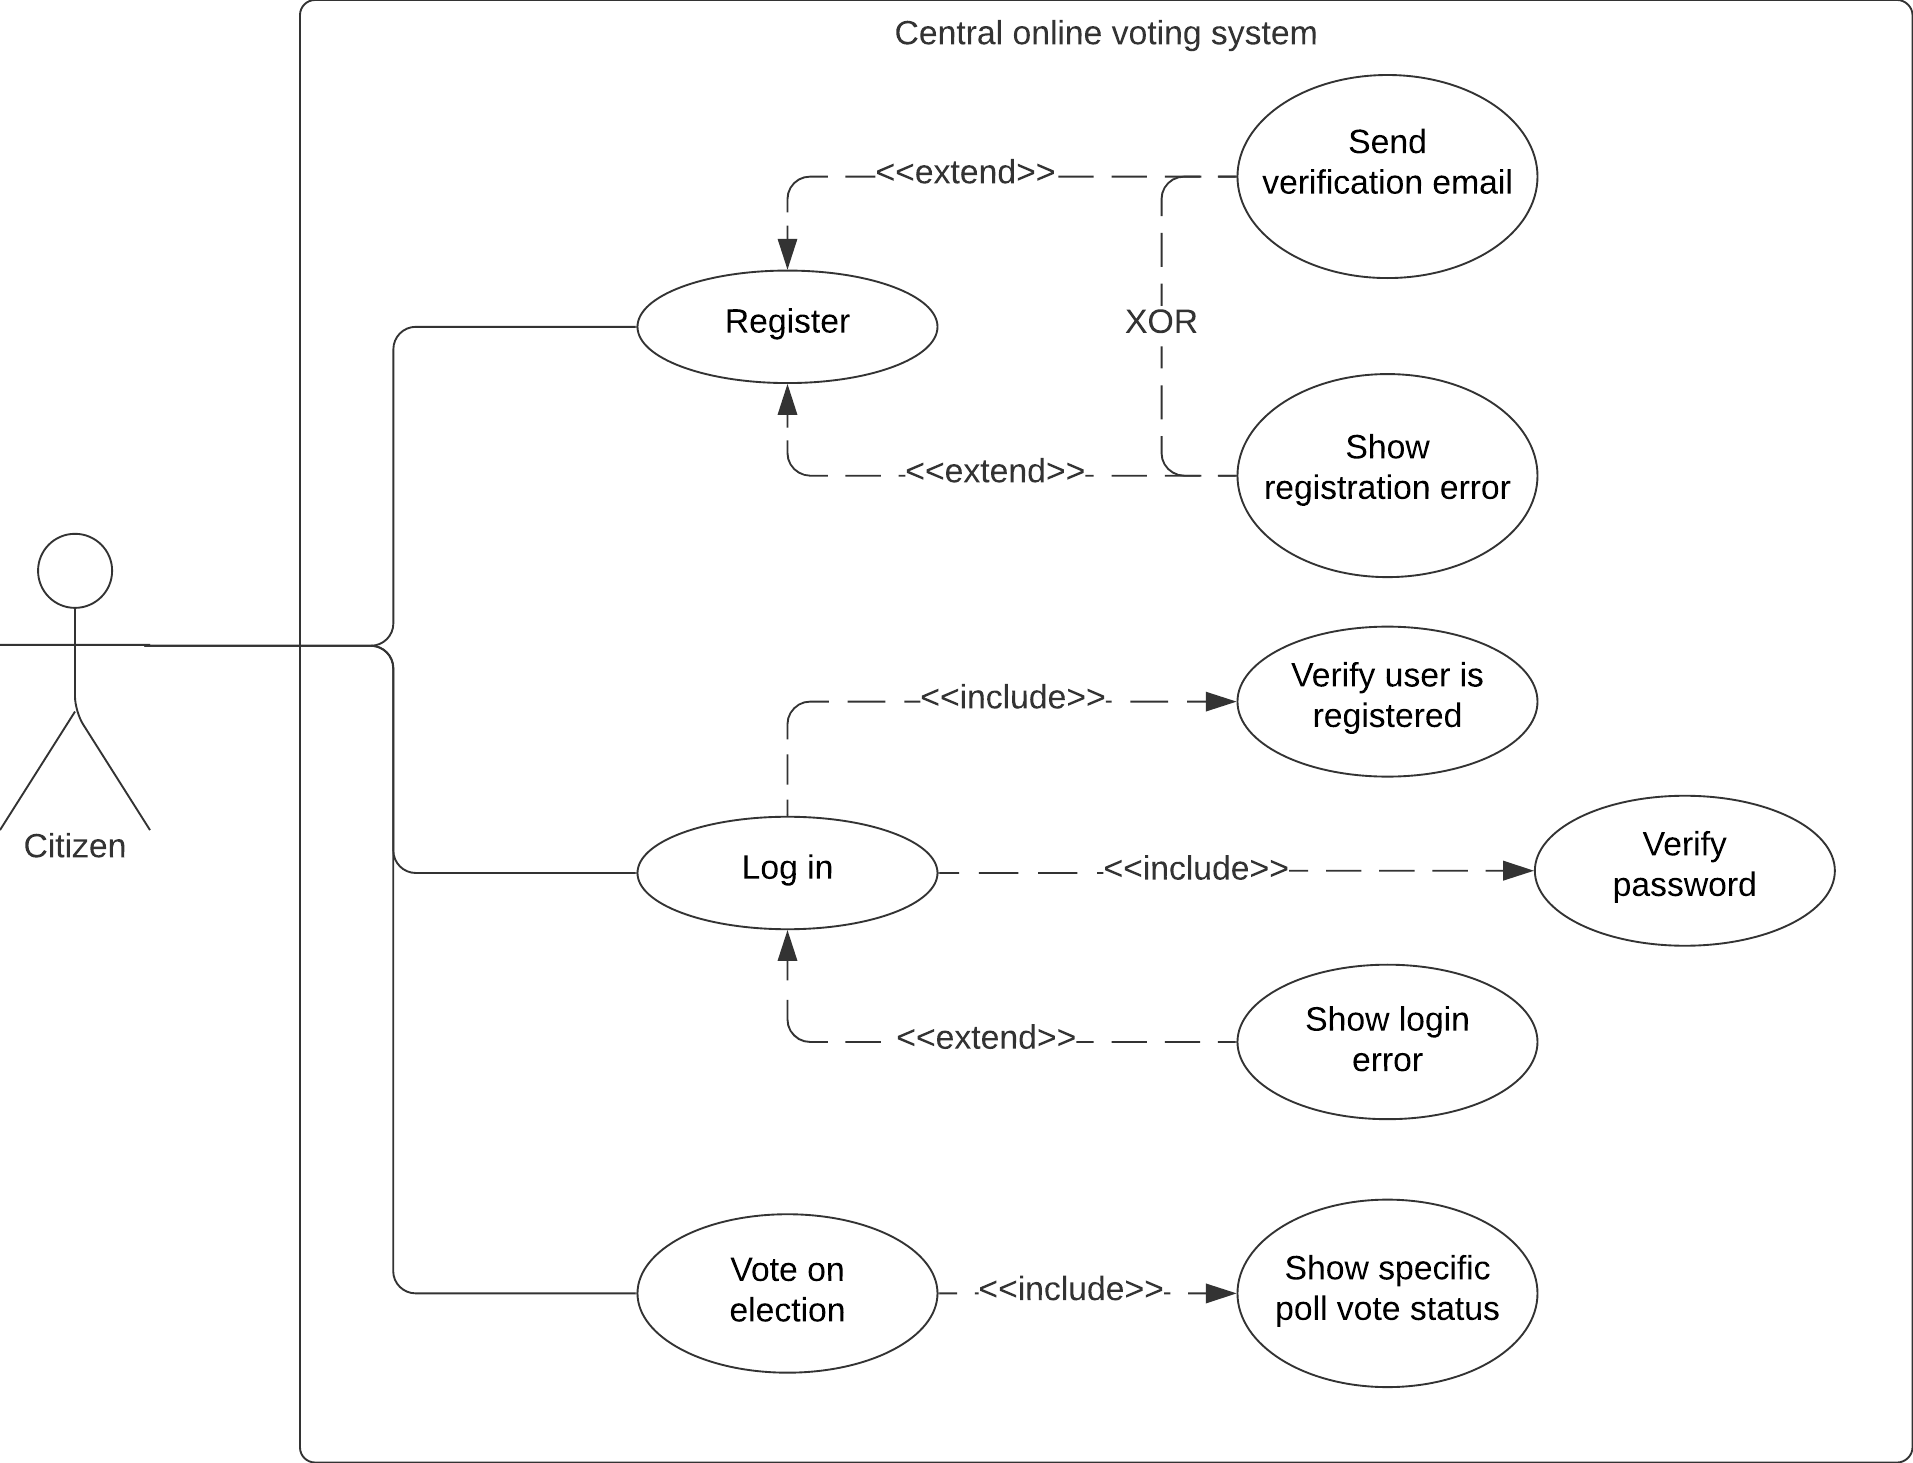
\includegraphics[width=\linewidth]{citizen_uml.png}
      \caption{Citizen use case UML for \Title}
      \label{fig:citizen_uml}
    \end{figure}

    Figure \ref{fig:citizen_uml} shows available use cases for a citizen. He can register and in that case he will receive an email, 
    or he can see some error regarding registration. A citizen can try to login, which will trigger checks if he is registered and that password matches.
    In case of any errors, he will see a message. 

    \subsection{Voter use case UML}
    \begin{figure}[h]
      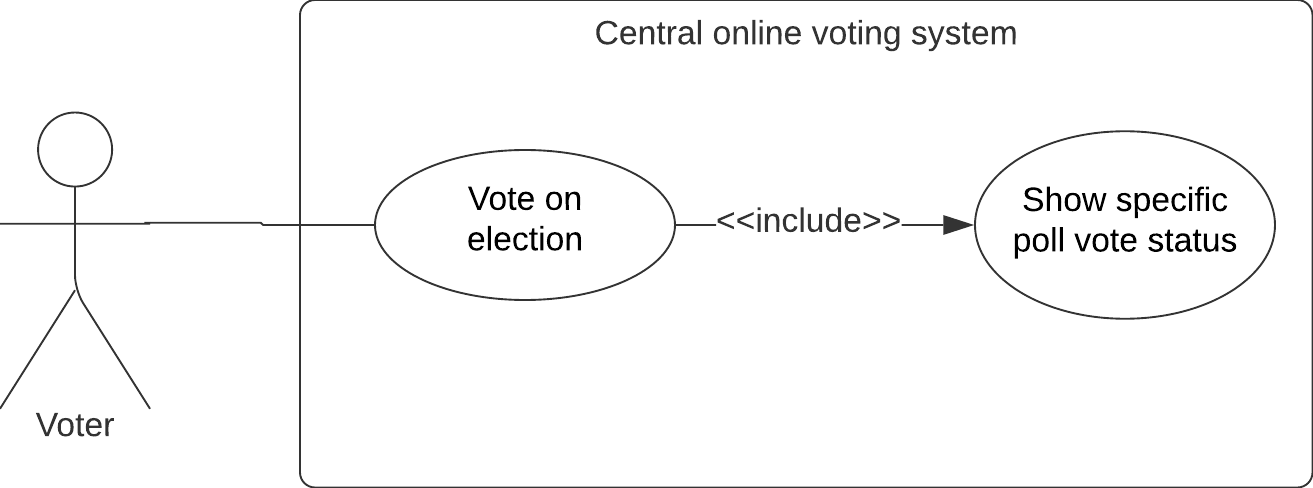
\includegraphics[width=\linewidth]{voter_uml.png}
      \caption{Voter use case UML for \Title}
      \label{fig:voter_uml}
    \end{figure}

    Figure \ref{fig:voter_uml} shows available use cases for a voter. A voter is a registered and successfully logged in user of the application.
    He can vote, and after that he will see status of his vote regarding every poll in the election, no matter if the vote is valid or not.
    However, even if a voter casted an invalid vote, he will not be able to vote again.

    \subsection{Ward administrator use case UML}
    \begin{figure}[h]
      \centering
      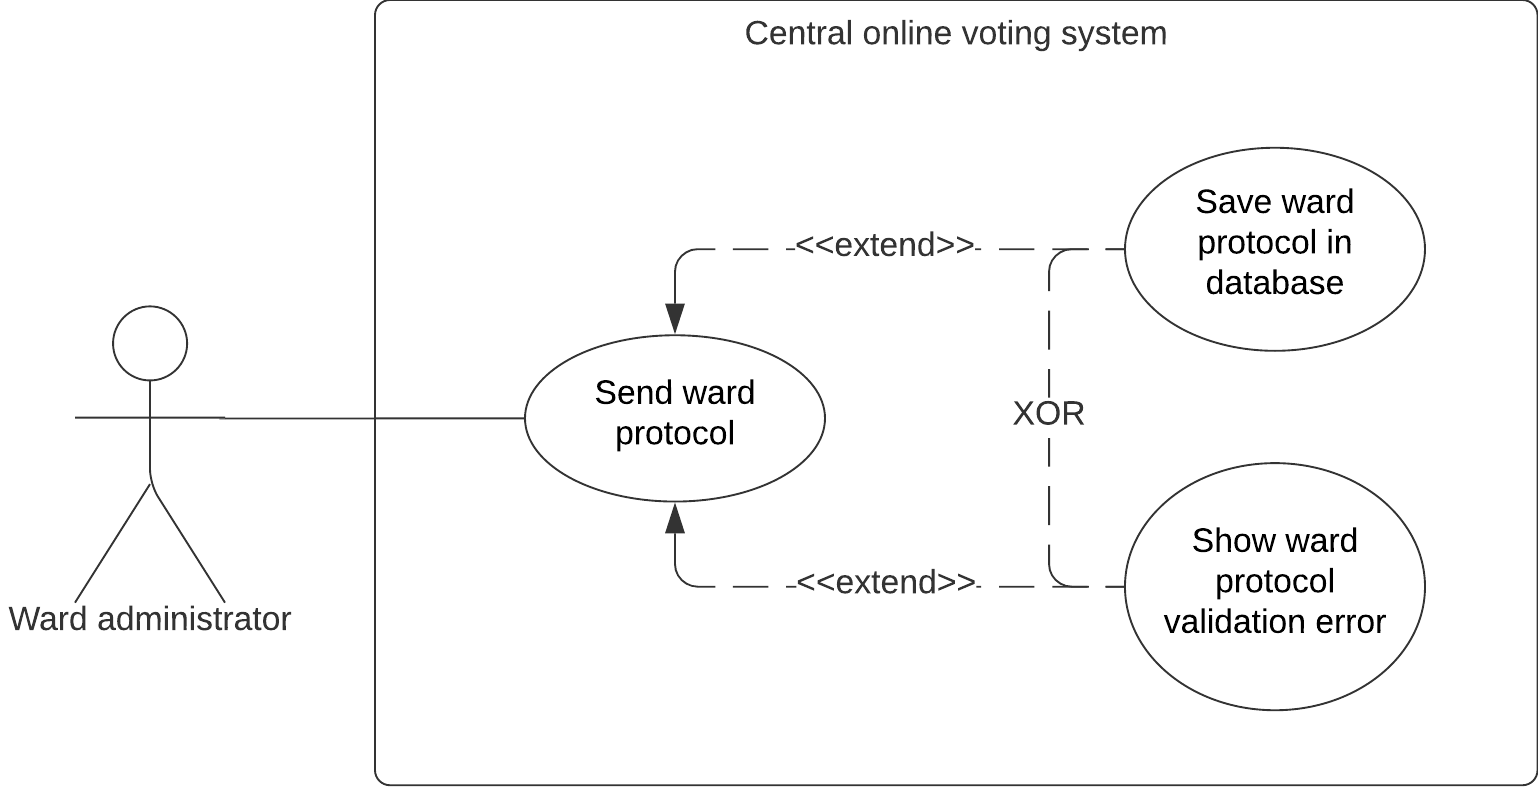
\includegraphics[width=0.65\linewidth]{ward_admin_uml.png}
      \caption{Ward administrator use case UML for \Title}
      \label{fig:ward_admin_uml}
    \end{figure}

    Figure \ref{fig:ward_admin_uml} shows available use cases for a ward administrator. A ward administrator can try to send a ward protocol.
    If anything is not correct in a protocol he tried to send, he will see a validation error, and the protocol will not be sent.

    \subsection{Committee administrator use case UML}
    \begin{figure}[h]
      \centering
      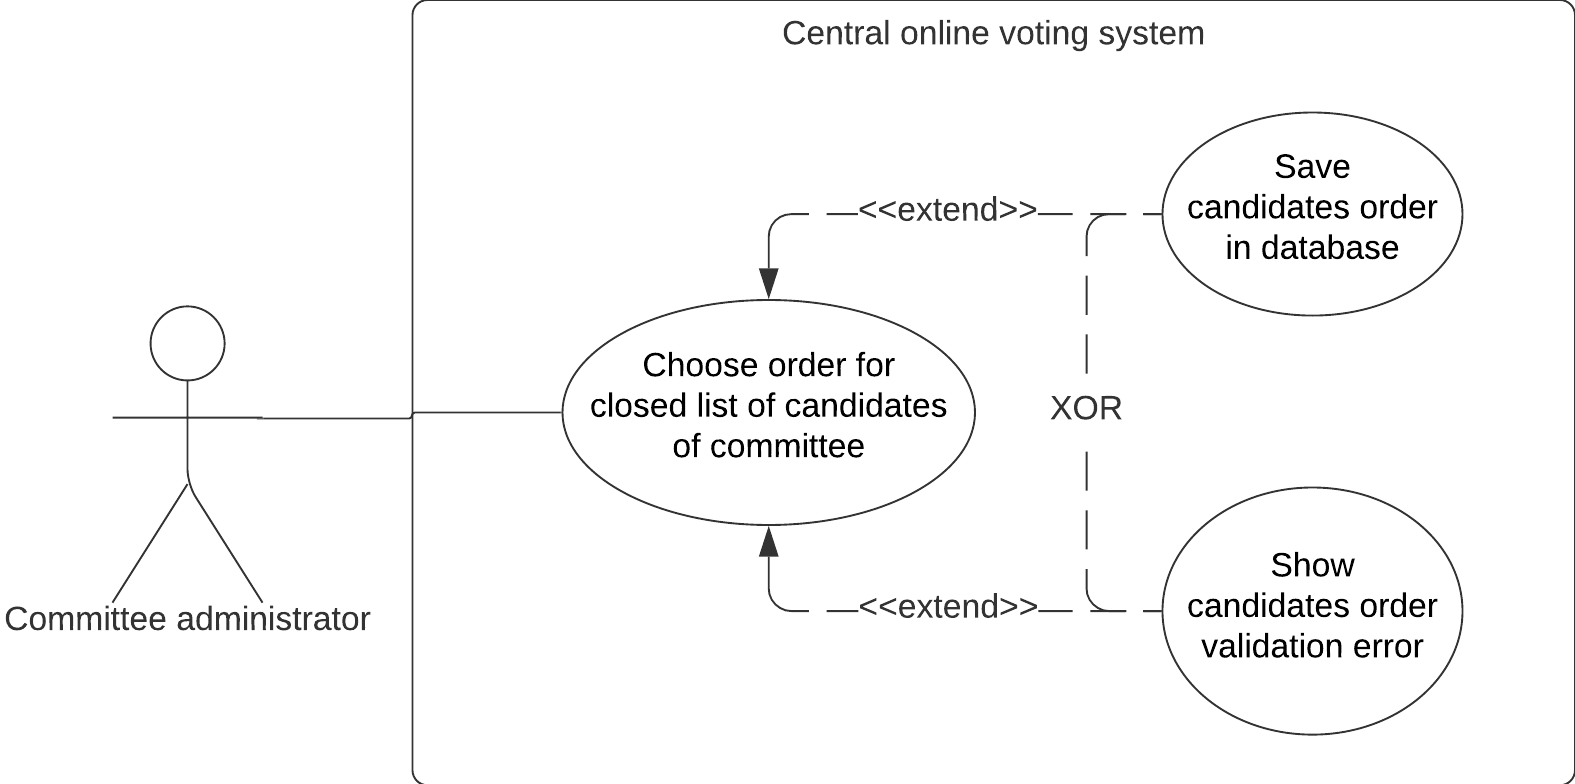
\includegraphics[width=0.65\linewidth]{committee_admin_uml.png}
      \caption{Committee administrator use case UML for \Title}
      \label{fig:committee_admin_uml}
    \end{figure}

    Figure \ref{fig:committee_admin_uml} shows available use cases for a committee administrator. A committee administrator can send closed list candidates' order.
    If anything is not correct in an order of candidates, he will see a validation error, and the candidates order will not be saved.
    \pagebreak

    \subsection{Administrator use case UML}
    \begin{figure}[h]
      \centering
      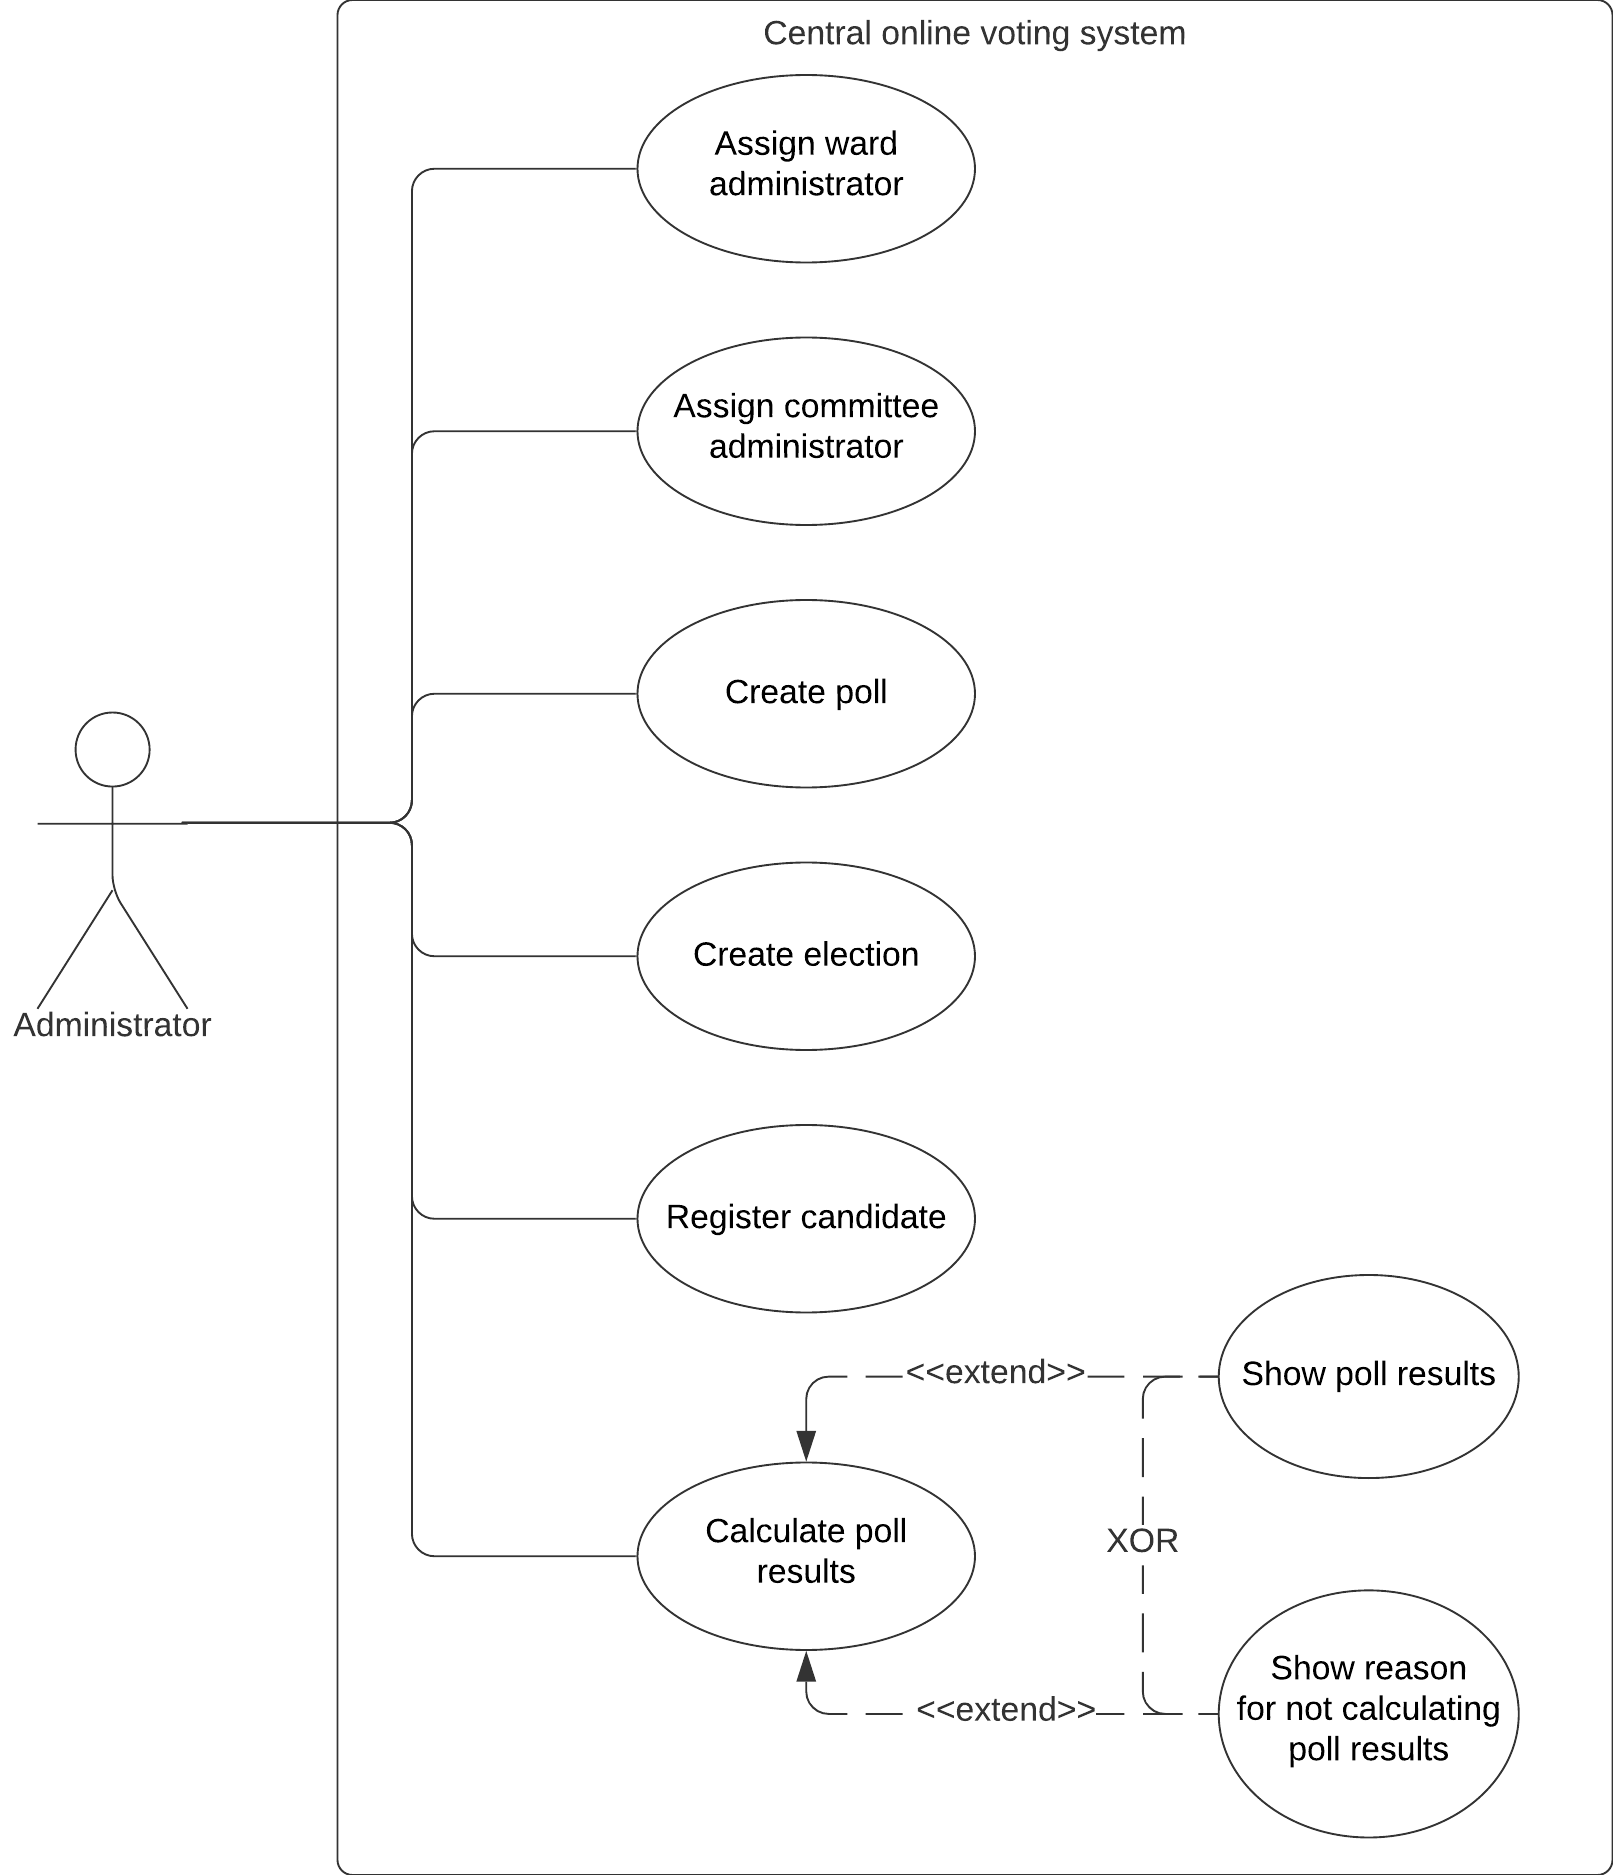
\includegraphics[width=0.8\linewidth]{admin_uml.png}
      \caption{Administrator use case UML for \Title}
      \label{fig:admin_uml}
    \end{figure}

    Figure \ref{fig:admin_uml} shows available use cases for an administrator. We assume that an administrator knows what he is doing, so there is no need to validate his choices.
    However, he has no power over how many protocols are sent from wards when he wants to calculate poll results. 
    Thus he will get appropriate message when he tries to calculate results of poll that is not ready to be calculated.

  \section{Description of tools}
    The application is developed in Java programming language with Spring Framework and Thymeleaf as template engine. 
    Data is stored in a MySQL database, and whole application is built with  Apache Maven build automation tool.

    \subsection{Java}
      It is an object--oriented programming language that requires Java Virtual Machine to run a program. 
      This allows Java applications to run on almost every device, regardless of it's operational system \cite{bib:horstmann2008core}.
      Java offers huge open--source ecosystem.

      \subsubsection{Alternative}
        C\# is also an object--oriented programming language, but it is used to develop software for Microsoft platforms \cite{bib:thai2003net}.

      Although there is no much difference in beginner level development between Java and C\#, I find C\# less convenient than Java,
      because I use machine with macOS operating system as my everyday work tool, and Java has huge support on Unix based system, compared to almost none support for C\#.

    \subsection{Maven}
      Apache Maven is a tool that is capable of building and managing any Java-based project. 
      It helps developers with dependency management, as it is able to download all necessary dependencies with almost no participation of developer.
      It is easy for beginners, as it is build lifecycles and syntax is easy to understand---all you need is artifact info of dependency that you want to include in your project, 
      and it will download and include dependency in project during install build lifecycle \cite{bib:maven}.

      \subsubsection{Alternatives}
        \paragraph{Gradle}
          It is also application build tool for Java-based projects. It is better than Maven for larger projects, thanks to better automation methods and better performance.
          Gradle is built with more experienced and demanding developer in mind~\cite{bib:gradle}.
        
        \paragraph{Ant}
          Ant is a powerful tool that allows developer to automate very complicated task, but this functionality is not cheap.
          It is a complicated to configure and it is being ousted by Gradle \cite{bib:ant}.

      \paragraph{} %I know it's probably not the way to achieve this result, but it works
      I chose Maven because I wanted to learn modern build technology that is common in the industry, but is suitable for beginners.

    \subsection{Spring}
      It is an open--source framework for Java platform. It focuses on delivering out--of--the--box core features for any kind of application, 
      so developers can focus on business logic of the application. 
      Aside from Spring Core, which provides easy dependency injection, Spring provides extensions in form of more or less independent modules, each available as it's own maven artifact \cite{bib:spring}.
      Spring Boot is an extension of Spring framework, which provides out--of--the--box configuration, and requires user to provide only application specific configuration.
      
      \subsubsection{Alternative}
        Because Spring is open--source framework, considered a standard in the industry for over 10 years, there is no other framework that is as feature--packed as Spring.
        One could make a case for .Net framework for C\# language, but it is developed and directed by Microsoft \cite{bib:thai2003net}, 
        whereas Spring is powered by community, and contains features required by that same community. 

      \subsubsection{Spring Security}
        Authentication and Authorization framework for Spring based applications. Provides quick protection of API exposed by application and
        integration with users in database. Allows for assigning users' roles, and managing accesses based on these roles \cite{bib:spring_security}.

      \subsubsection{Spring Web MVC}
        It is designed around front controller pattern, and helps developers follow the Model--View--Controller design pattern.
        It coordinates flow of request processing performed by configurable delegate components \cite{bib:spring_web_mvc}.
      
      \subsubsection{Spring Data JPA}
        Spring implementation of JPA contract, powered by Hibernate. Reduces hugely boilerplate code that is associated with querying database,
        especially with Repository interface custom finder methods \cite{bib:spring_data_jpa}.

    \subsection{Thymeleaf}
      Modern server-side Java template engine resolver. 
      It converts HTML files with Thymeleaf--specific dynamic attributes based on model attributes provided by developer through Spring MVC framework \cite{bib:thymeleaf}.
      
      \subsubsection{Alternative}
        There are not many pure alternatives when it comes to template resolvers. 
        Java Enterprise Edition comes with JSP, which is not pleasant to use, and is considered obsolete.
        It definitely does not provide level of integration with Spring MVC framework as much as Thymeleaf does.

  \section{Methodology of design and implementation}
    Base of every application is a well designed database schema. 
    Once schema is designed with required functionalities of application in mind, and with space for extensibility predicted,
    it makes development not only go faster and more efficient, but also more pleasant for a developer.

    With proper database schema, we have to consider what is the best way for user to use our application---through web browser or application?
    Because application is meant to be nation--wide, 
    and there is a web browser on perhaps every computer with internet connection---which is necessary for application to work---web application is the way to go.
    
    When designing web application, we have to decide how we want to achieve end result---presenting view to application user.
    There are two most common approaches when it comes to Spring application:
    \begin{itemize}
      \item Exposing REST API from Spring application, that contains all of business logic and create another application, that consumes that API and interacts with the user in any way desired.
      \item Keep view rendering on server side and expose pure html to the user.
    \end{itemize}
    I chose the second option, because it is not the most important thing for \Title\ to be pretty and responsive, I wanted to focus on a backend side of the application.

    Once view presenting is established, we want to consider how we want to design architecture of the application.
    I can see two approaches in choosing the architecture: basing on application requirements or basing on technology used in application.
    Because Spring provides a whole framework dedicated to the MVC design pattern, and also it is widely used in the industry, I chose to develop the application in that manner
    rather than choosing architecture basing on application requirements. 
    My application is not large enough to be hugely impacted by bad architecture. I could only harm my project by using some fancy architecture.

\chapter{External specification}
  \section{Types of users and cockpits}
    \subsection{Overview}
    In order to secure the application from unauthorized access  I divided the application into four main cockpits:
    \begin{itemize}
      \item Voter cockpit,
      \item Administrator cockpit,
      \item Ward administrator cockpit, and
      \item Committee administrator cockpit.
    \end{itemize}
    Each cockpit requires a specific user role to access it's website.
    In order to have access to anything we have to be an authenticated (active, successfully registered) user with assigned role that gives us permission for certain cockpits.
    A guest---not registered user---is only allowed to register or login.

    \subsection{Voter cockpit}
    \label{subsec:voter_cockpit}
    A user with a role of a voter is able to vote for election and see election results after the election is closed.
    In case of voting a user is be able to vote on a poll only once without any exception.

    \subsection{Administrator cockpit}
    A user with a role of an administrator is able to create essential data---wards, polls, committees etc. as well as granting certain roles to certain users.
    An administrator is not be able to interfere in a ward or committee administration other than choosing its administrator.
    Moreover administrator is the one that triggers polls results calculation.

    \subsection{Ward administrator cockpit}
    A user with a role of a ward administrator is able to manage only his assigned ward. Under no circumstances he is able to manage other wards.
    In a ward administrator cockpit he is able to enter a  protocol from a ward for each poll during an election.

    \subsection{Committee administrator cockpit}
    A user with a role of a committee administrator is able to manage only his assigned committee. Under no circumstances he is able to manage other committees.
    In a committee administrator cockpit he is able to choose an order of committee candidates in a closed list. 
  
  \section{Software requirements}
    In order to run the application, you have to have Java 12, Maven 3.6.X installed and MySQL 8.0.17 running on the application server, 
    make sure that \lstinline[language=bash]|java| and \lstinline[language=bash]|mvn| executables are in PATH environment variable.

  \section{Installation procedure}
    First, you have to adjust the database connection properties in \lstinline|APP_ROOT/src/main/resources/application.properties|. Exemplary properties are already provided in the source code.
    Also in that file, you have to specify the connection properties to the SMTP server to be able to send e-mails. Exemplary SMTP server connection properties are also provided.
    In order to build project, you have to execute Maven install lifecycle \lstinline[language=bash]|mvn install| in \lstinline|APP_ROOT| directory.
    This lifecycle will generate \lstinline[language=bash]|ballotbox-0.0.1-SNAPSHOT.jar| jar file in \lstinline|APP_ROOT/target| directory.
    To run application you have to execute \lstinline[language=bash]|java -jar APP_ROOT/target/ballotbox-0.0.1-SNAPSHOT.jar|. 
    Application server will listen on PORT 8080 by default. 
    
  \section{Activation procedure}
    Users' roles definitions are loaded into a database on first server startup if they do not exist in the database already.
    Same behaviour with the default admin user with password `nimda'---it is in the database on the first startup.
    To secure the application you have to register a proper user which is meant to be an administrator, and execute  following query in the database:

    \lstinline[language=sql]|INSERT INTO users_roles(user_id, role_id) values (ADM_ID, ROLE_ID);|
    Where \lstinline[language=sql]|ADM_ID| is an id of a desired administrator in table `user', and \lstinline[language=sql]|ROLE_ID| is an id of a row with a column name equal to \lstinline[language=sql]|``ROLE_ADMIN''| in table `role'---1 by default.
    That is the procedure you should follow when you want to add an administrator to the system.
    After that you should delete the predefined admin user from table user, with following query:

    \lstinline[language=sql]|DELETE FROM user WHERE username='admin';|

  \section{User manual}
    \subsection{Voter manual}
      A Voter can access voting page at the root endpoint of the application---\mbox{\lstinline|HOST:PORT|.}
      After clicking \lstinline|show all elections|, a user can choose election on which he wishes to vote in.
      After clicking on vote button, he can cast a vote in all polls available in this election.
      \pagebreak
      There are two types of voting methods. One is a single choice vote---voter can mark a checkbox next to candidate he wishes to vote on.
      \begin{figure}[h]
        \centering
        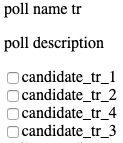
\includegraphics[width=0.3\linewidth]{single_choice_vote_screenshot.png}
        \caption{Single choice vote screenshot}
        \label{fig:single_choice_vote_screenshot}
      \end{figure}

      Second type of voting is preference voting, in which voter can mark candidates by his choice of preference:
      1 for a candidate of his first choice, 2 for his second favourite candidate and so on.
      \begin{figure}[h]
        \centering
        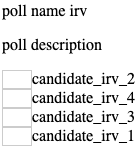
\includegraphics[width=0.3\linewidth]{preference_vote_screenshot.png}
        \caption{Preference vote screenshot}
        \label{fig:preference_vote_screenshot}
      \end{figure}

      Description provides user with specific instructions on how to vote on a specific poll. If user does not follow the instructions, vote is invalidated, and voter cannot vote again.
      After casting a vote, user gets information on status of his votes - if vote is validated or not, and if not, why.
      After election is finished and results are calculated, voter can see results of poll after clicking on results button.
      He will get information about how many valid votes were casted in a poll, and who are the winners of that poll.

    \subsection{Committee administrator manual}
      Committee administrator can access committee management page after going to \lstinline|HOST:PORT/committeepanel| endpoint of the application.
      After that, he can choose which committee that he is an administrator of he wishes to manage.
      Then, he can set closed list order of that committee, required for D'Hondt method.
      If he makes any error, he will be displayed appropriate message, and order will not be saved---it will be held at previous stage.

    \subsection{Ward administrator manual}
      Ward administrator can access ward management page after going to \lstinline|HOST:PORT/wardpanel| endpoint of the application.
      After that, he can choose which ward thet he is an administrator of he wishes to manage.
      Then, he can send specific poll protocol from that ward.
      If administrator makes any error in protocol, he will be displayed appropriate message, and protocol will not be sent.

  \section{System administration}
    In order to access administrator cockpit, we should go under \lstinline|HOST:PORT/panel| URL in the browser, when logged in as user with administrator rights.
    \begin{figure}[h]
      \centering
      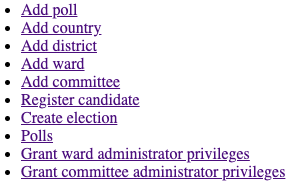
\includegraphics[width=0.5\linewidth]{admin_panel_screenshot.png}
      \caption{Administrator panel screenshot}
      \label{fig:admin_panel_screenshot}
    \end{figure}

    On figure \ref{fig:admin_panel_screenshot} we can see all available actions for administrator.
    \subsection{Add country}
      Crete a country with typed in name. 

    \subsection{Add district}
      Create a district with typed in name, and select country that owns created district.

    \subsection{Add ward}
      Create instance of real ward in district - place where people come to vote. 
      Select district that owns created ward.

    \subsection{Grant ward administrator privileges}
      Choose ward and existing user. Chosen user will be ward administrator of chosen ward. One user could be administrator of many wards.

    \subsection{Add committee}
      Create a committee with typed in name.

    \subsection{Grant committee administrator privileges}
      Choose committee and existing user. Chosen user will be committee administrator of chosen committee. One user could be administrator of many wards.

    \subsection{Add poll}
      Create poll. Type in unique name and short description. Choose date in which poll will be available to vote.
      Choose poll scope---citizens from which wards can place a vote in this poll.
      For example, if you choose country scope, citizens from all wards that belong to all districts that belong to country chosen will be able to vote in this poll.
      Same applies to district scope---citizens from all wards that belong to chosen district will be able to vote in this poll.
      Next, select voting method. It is a method in which results will be calculated, but also it will determine how voters can cast their vote.
      There are four available methods, each with constraints:
      \begin{itemize}
        \item Winner takes all---Number of seats to fill must be 1, voter can mark only 1 candidate. Candidate with higher number of votes overall wins.
        \item Two round---Number of seats to fill must be 1, voter can mark only 1 candidate. Poll is resolved only if one candidate has over half of all votes.
        \item Instant runoff voting---Number of seats to fill must be less than number of candidates participating (type in desired number),
        voter can mark maximum of available candidates (type in desired number).
        Voter will vote on candidates based on his number of preference for each candidate---1 for highest preference, 2 for slightly lower and so on.
        \item D'Hondt method---Number of seats to fill must be less than number of candidates participating (type in desired number),
        voter can mark only 1 candidate. Results of poll will be calculated using D'Hondt method, using closed lists from committees, provided by committee administrators.
      \end{itemize}
      \begin{figure}[h]
        \centering
        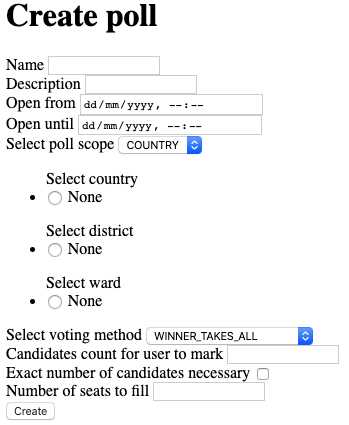
\includegraphics[width=0.4\linewidth]{add_poll_screenshot.png}
        \caption{Add poll screenshot}
        \label{fig:add_poll_screenshot}
      \end{figure}

    \subsection{Register candidate}
      Select an existing user and register him as a candidate in a poll, as candidate from chosen committee.

    \subsection{Create election}
      Create an election from existing polls. Voter will have only one chance to vote on polls contained in an election.

    \subsection{Polls}

      \begin{figure}[h]
        \centering
        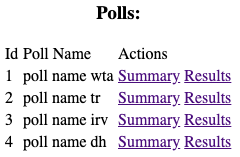
\includegraphics[width=0.4\linewidth]{polls_screenshot.png}
        \caption{Polls menu screenshot}
        \label{fig:polls_screenshot}
      \end{figure}

      Opens available polls menu. For each poll we have two options: Summary and Results.

      \subsubsection{Summary}
        Shows if poll is active (can be voted on), and how many votes were casted over the internet.

      \subsubsection{Results}
        Calculates and shows results of chosen election. Results will not be calculated if poll is still active, or if any ward did not send the protocol.
        Once results are calculated they are stored in database and will not be calculated again---there is no need to.

  \section{Security}
    There are two layers on which application is protected from misuse. 
    First checks if user has access to requested resource, second makes sure that user cannot affect data in an unwanted way.

    \subsection{Access check}
      Application is protected against unauthorized access with help of Spring Security. It handles authentication and authorization following only guidelines of the developer.
      Every registered user is granted a `USER' role, which permits him to access every resource at root URL (\nameref{subsec:voter_cockpit}).
      After user is authenticated---he is confirmed to exist in database, to be activated and password provided matches that in a database---his roles are checked.
      If and only if his set of roles includes that required by the resource, the authorization filter passes the request forward to the controller.
      It's configured in the \lstinline|SecurityConfiguration| class.

    \subsection{Business logic security}
      API calls which may affect data written to database are additionally protected against misuse of the application, which may lead to taking advantage of it.
      Whenever there is a call that should be protected by some business logic, before it performs anything, 
      it checks whether user that makes that call can perform desired action. If not, it returns with message why action was not performed. 
      
      Protection against casting a second vote in an election is a great example to understand how business logic security works.
      Given an authenticated and authorized user, let's assume that he wants to cast a vote in an election. 
      Here are steps performed to secure the application from misuse:
      \begin{enumerate}
        \item Regular checks if election from url exists.
        \item Check if user's location (ward, district and country) matches polls in the election.
        \item Check if user has not already voted in this election.
        \item Check if polls in the election are currently active.
      \end{enumerate}
      Those checks are common for displaying the vote page and posting a vote form.
      Apart from those standard checks, posting a vote form has some additional checks:
      \begin{enumerate}
        \item Check if polls posted in a form actually belong to requested election.
        \item Validation of every vote on a poll. In case of any unwanted or corrupted data, vote is invalidated.
      \end{enumerate}
      But before that checks, all polls from that election are marked as voted by the user posting the vote.
      In order to fulfil requirement that user's vote should be untraceable, few actions are worth mentioning:
      \begin{itemize}
        \item All polls from requested election are added to set of polls that user has voted in.
        \item Vote itself has no information about who casted it and when---vote is impersonal, 
          there are no application logs at any level regarding casting a vote, 
          there is no timestamp in the database that could connect when vote was created and marking poll as voted by a user.
      \end{itemize}

\chapter{Internal specification}
  \section{Concept of the system}
    \begin{figure}[t]
      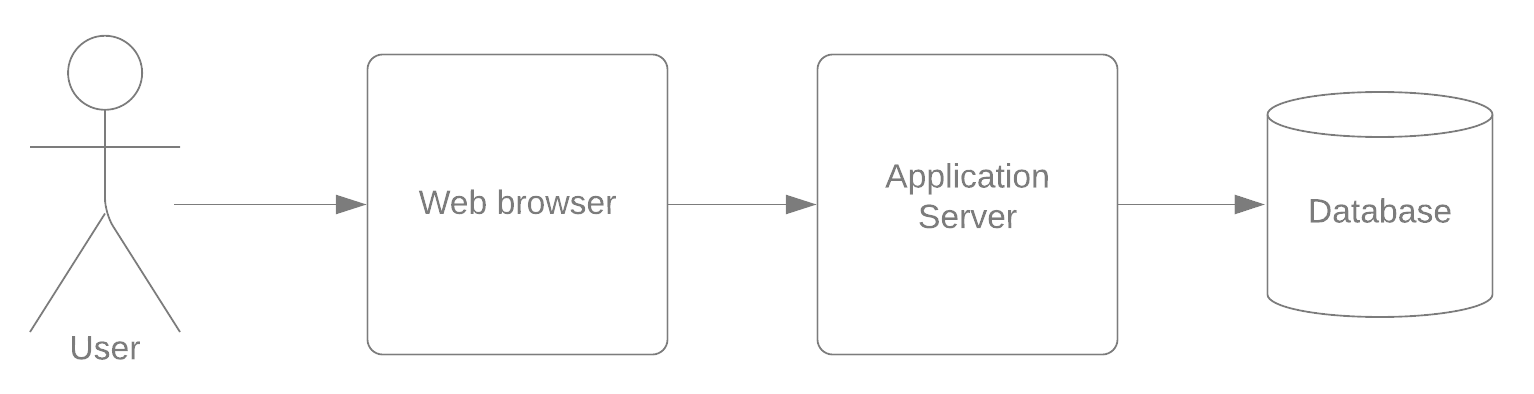
\includegraphics[width=\linewidth]{system_concept.png}
      \caption{Concept of the system}
      \label{fig:system_concept}
    \end{figure}

    
    A user communicates with the system via a web browser. 
    A web browser sends HTTP requests to the application server which constructs the response using resources available in a database (Fig. \ref{fig:system_concept}).
   % \pagebreak

  \section{System architecture}
    Figure \ref{fig:architecture_diagram} shows architecture of the application. 
    A user interacts with a web browser and his actions trigger communication of the browser with the application server via HTTP.
    Those requests are passed through security filters of Spring Security, which check if user is authenticated and authorized to fetch the resource he requests.
    After that, all requests hit dispatcher servlet, which delegates request to it's specific request controller.
    Repository layer provides data available directly in the database, 
    while service layer performs some additional logic, which is not available in the repository logic (some simple filtering of fetched data).
    Repository talks to the database with help of Hibernate, JPA implementation used by Spring Data JPA. 
    Controller connects all data provided to it by service or repository layer into business logic, and constructs a view model for HTTP request.
    This view model is passed to template engine, 
    which applies this view model to specific view template (information regarding which template is also mentioned in view model), 
    and constructs HTTP response for this template.
    This response comes back to security filters, which send response back to web browser.
   % \pagebreak
    \begin{figure}%[p]
      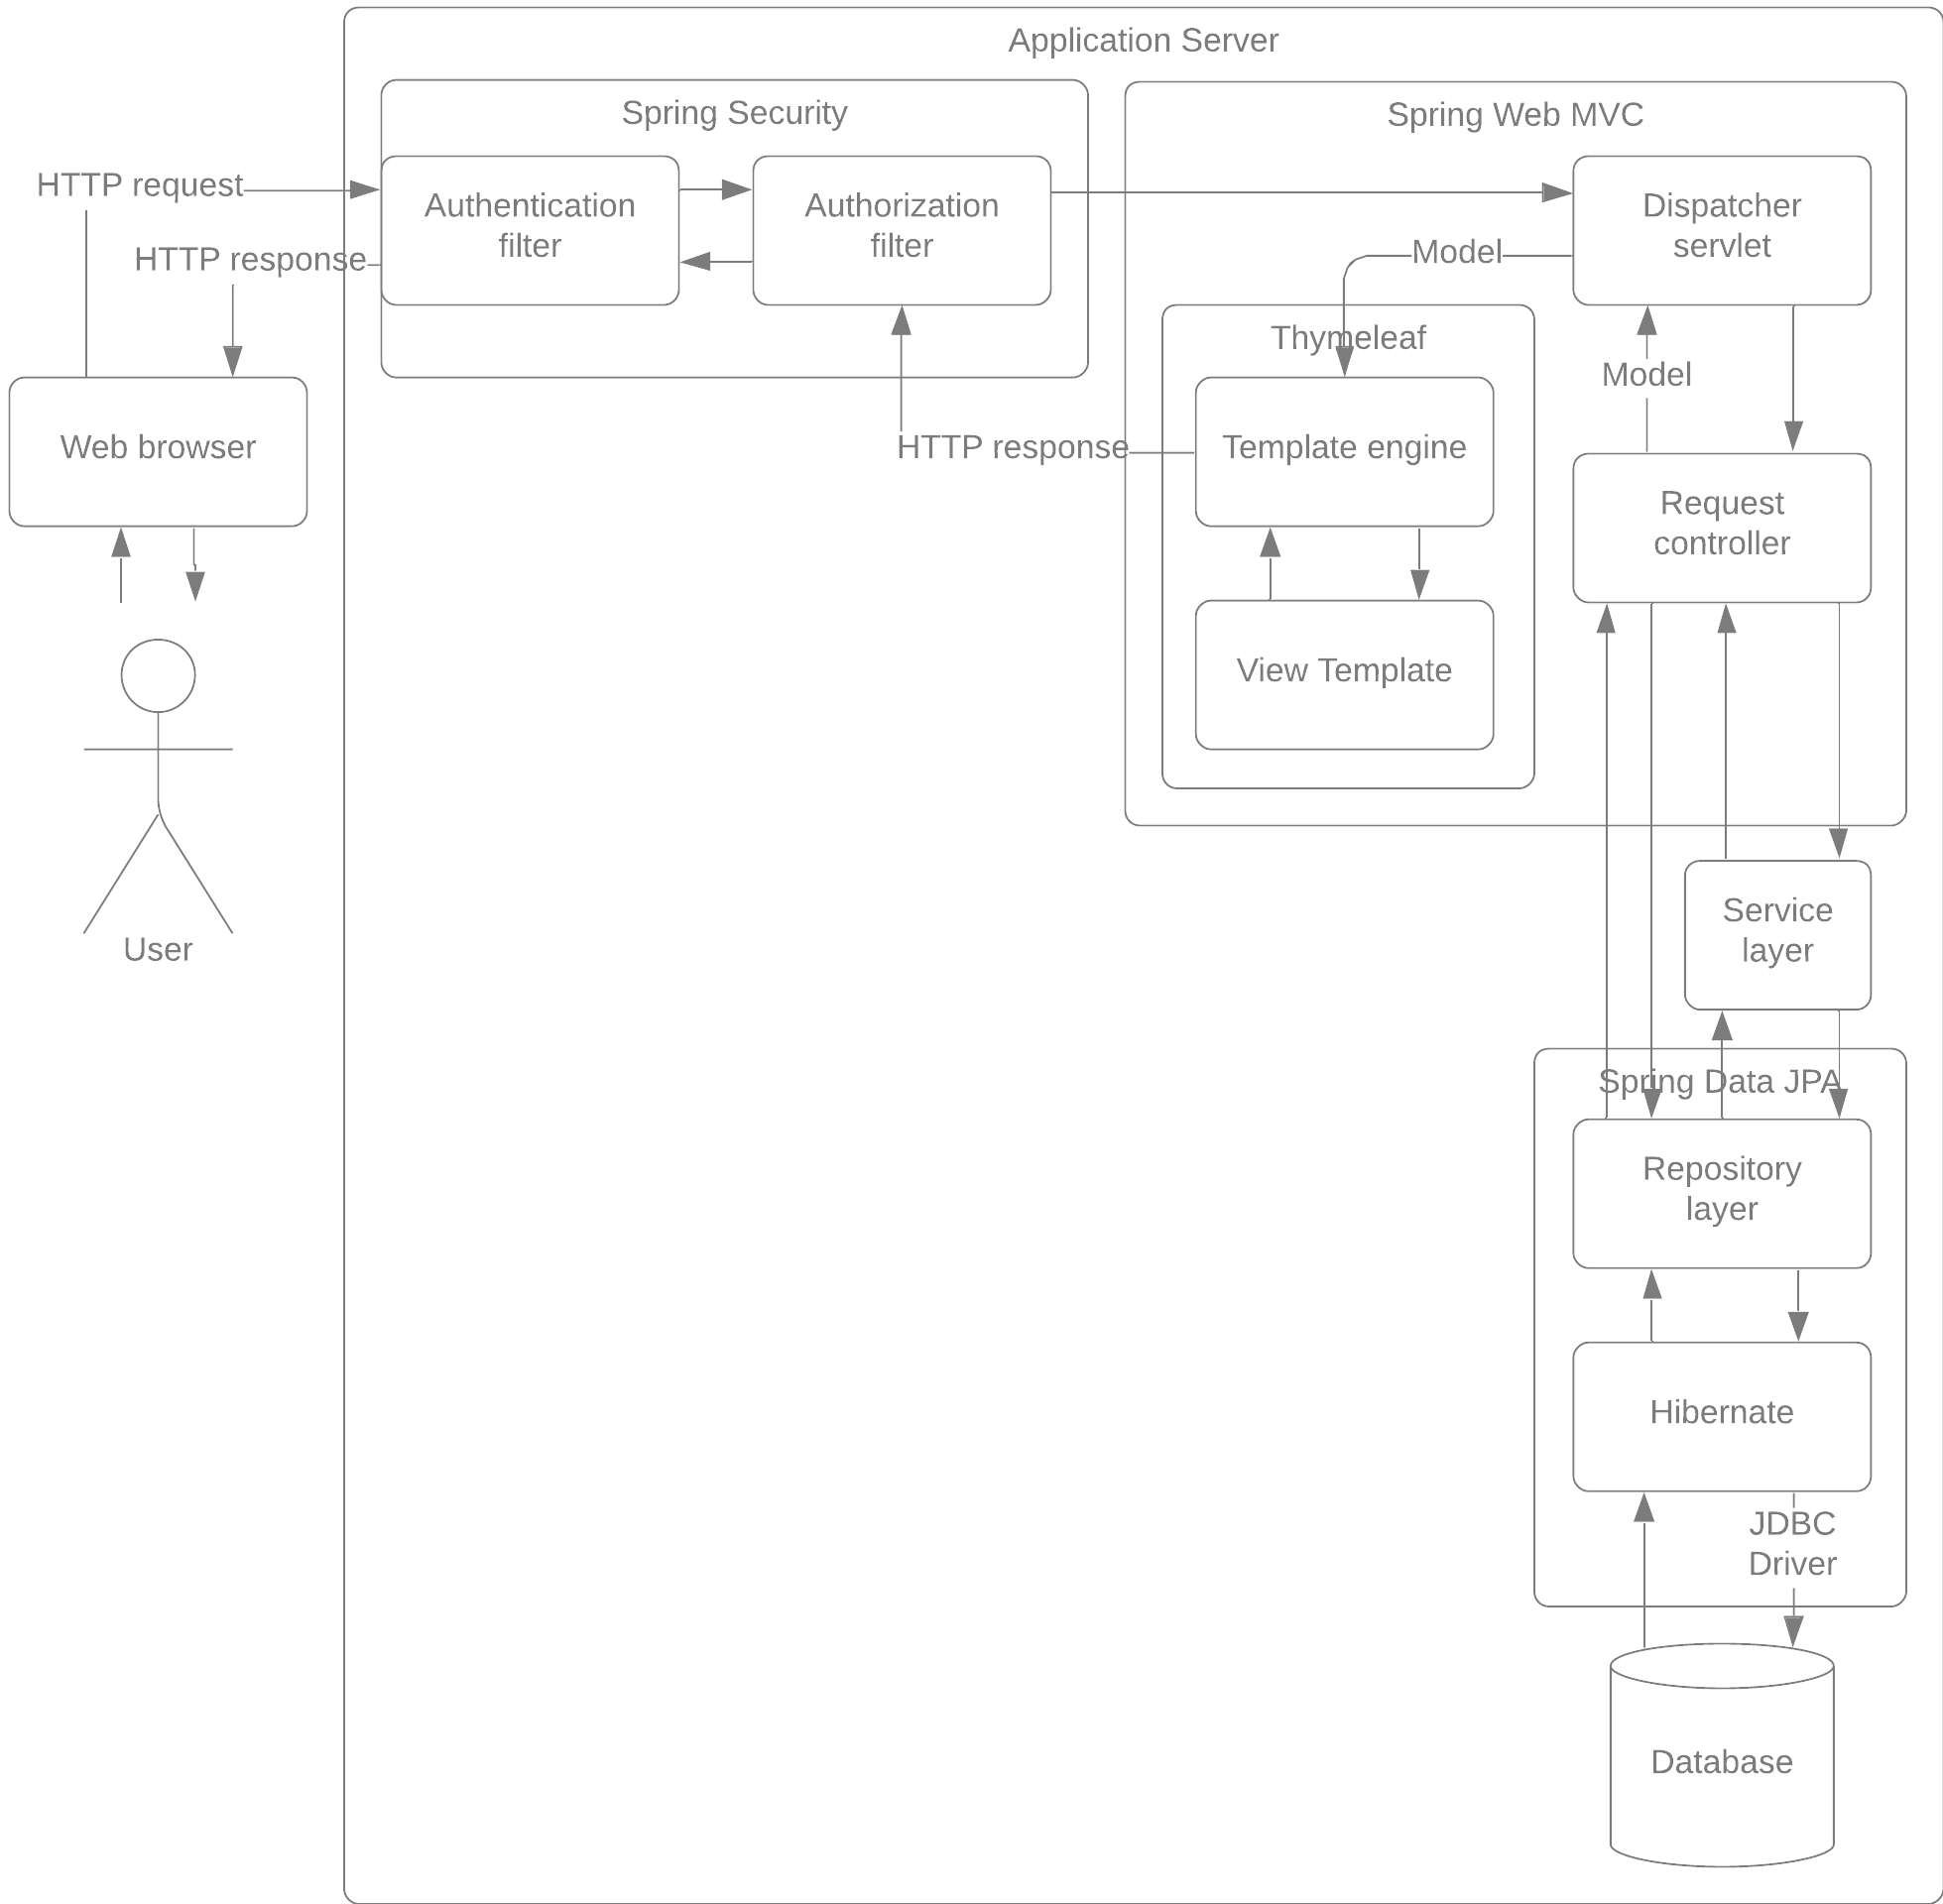
\includegraphics[width=\linewidth]{architecture_diagram.png}
      \caption{Application architecture}
      \label{fig:architecture_diagram}
    \end{figure}
 %   \pagebreak

  \section{Data structure}
  \ksremark{Pusty podrozdział – brak tekstu :-)}
  
   
  
    \begin{figure}%[p]
      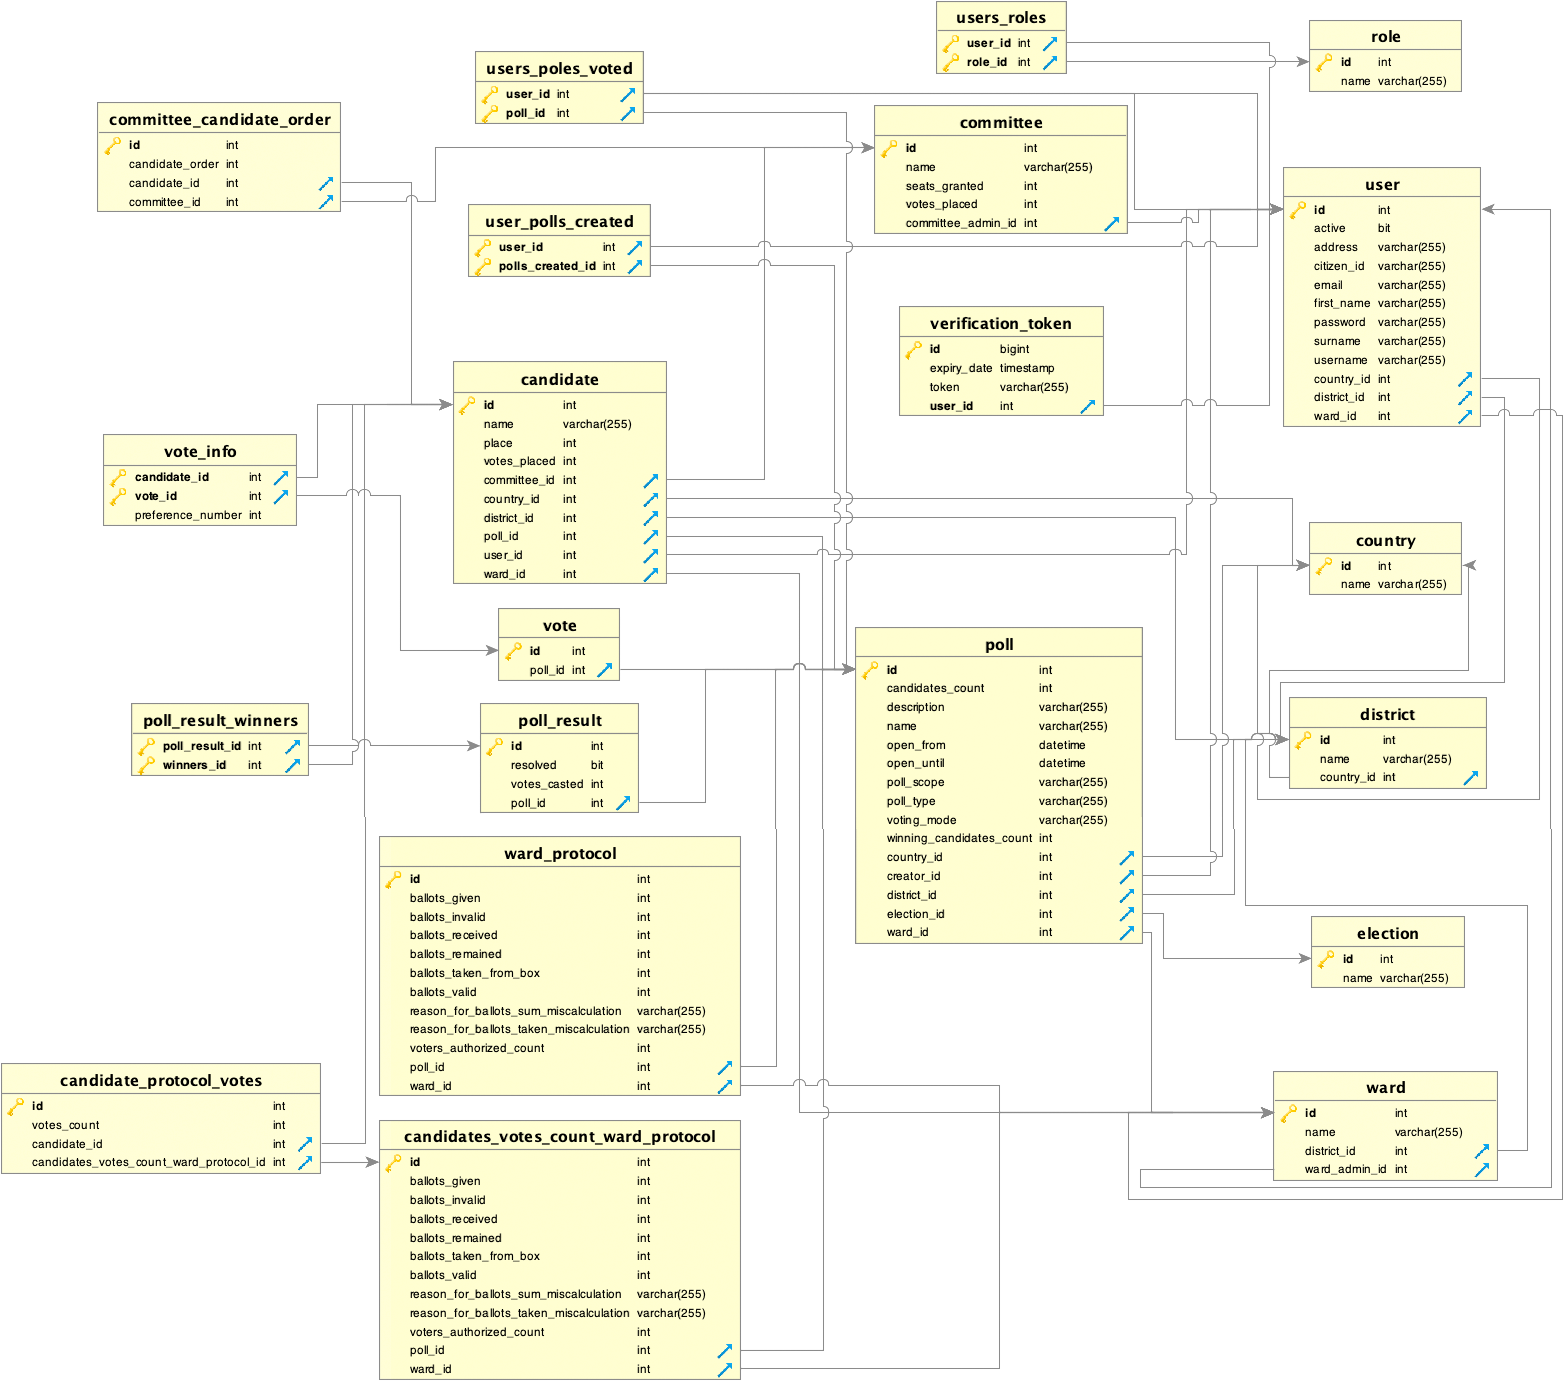
\includegraphics[width=\linewidth]{erd.png}
      \caption{Entity-Relationship Diagram of the data structure used by the application}
      \label{fig:erd}
    \end{figure}
  %  \pagebreak

  \section{Implementation of the application}
    \subsection{Entity}
      An entity class is a representation of a table in a database.
      It can be treated as implementation of business data model, which is used to achieve some business result.

      Apart from standard Java syntax, there are some annotations related to JPA in an entity class:
      \begin{itemize}
        \item\lstinline|@Entity|---marks class as entity. It will be represented in database as a table.
        \item\lstinline|@Id|---marks class field as primary key for table.
        \item\lstinline|@GeneratedValue|---determines strategy for generating this value when writing to database in case of null.
        \item\lstinline|@ManyToOne|---marks class field as many to one relationship with another entity. 
        It will store primary key of target entity in table of this entity.
        There is a twin annotation to this one, \lstinline|@OneToMany| for entity on the other side of this relation.
      \end{itemize}
    
    \subsection{Repository}
      A repository is an interface that allows a developer for interaction with objects stored in a database.
      Spring Data JPA provides out--of--the--box implementation of a CRUD repository.
      A \lstinline|@Repository| annotation allows Spring to identify such interface, create implementation of it and hold it in the context.
      It is easily extensible with help of custom finder methods, which search and filter based on name of the method declared in an interface.

    \subsection{Component}
      In order to help Spring identify dependency classes eligible for DI, we can annotate such classes with any derivative of \lstinline|@Component| annotation.
      When spring is scanning for components, \lstinline|@Component| annotated class will be treated as component, thus an object of such class will be created and held in the context.
      There are several derivatives of \lstinline|@Component| annotation, which serve the same purpose, but are named differently for simpler understanding of class role and behavior.
      Examples of \lstinline|@Component| specialized annotations:
      \begin{itemize}
        \item \lstinline|@Service|
        \item \lstinline|@Controller|
        \item \lstinline|@Repository|
      \end{itemize}
      If needed, those dependencies can be injected using \lstinline|@Autowired| annotation.
      It looks for dependency of matching type as field under annotation, and assigns desired object to class field after owner object construction.

    \subsection{Controller}
      A controller is a class that can process HTTP requests. It is annotated with \lstinline|@Controller| annotation, along with \lstinline|@RequestMapping| annotation, 
      which value determines what URL this controller responds to.
      As HTTP has few methods that determine type of request under certain URL, controller class method annotations like \lstinline|@GetMapping| and \lstinline|@PostMapping|
      map HTTP method to class method, which that request triggers.

      There are many arguments that mapping method can take that give developers additional tools for processing HTTP request.
      This application uses \lstinline|Model| class as method argument to create a model passed to template.
      In case of POST HTTP method, we can use \lstinline|BindingResult| class in method argument to get information about form that was sent with HTTP request.
      Controller decides which template should be used by returning template location in \lstinline|String| type.
      This location is relative to folder \lstinline[language=bash]|APP_ROOT/src/main/resources/templates| by default.

    \subsection{View template}
      A view template is a HTML file with additional tags and attributes which are parsed by Thymeleaf after populating template with a model.
      This means that any errors in template file are runtime error, as template is parsed at the end of HTTP response generation flow \ref{fig:architecture_diagram}.

  \section{Applied design patterns}
    While many design patterns may be useful in big projects, there was no need to introduce any sophisticated methods of organizing application layers and communication.
    I kept it simple, and it worked for me. 

    I based my architecture on MVC architectural pattern. 
    I chose it because of wide use in the industry and the fact that there is a separate dedicated Spring framework to help developers when using that pattern. 

    All dependencies between classes are managed according to Dependency Injection (DI) design pattern. It is best seen in \lstinline|PollResultController| class. 
    This controller uses a defined interface of calculation services, which implementations are provided by application context, first given a specific poll to be calculated.
    It is also visible in almost every service class of the application (see \lstinline|CommitteeServiceImpl| for example). 
    Services use repository interfaces, which are constructed by Spring Data JPA, and injected from application context with help of \lstinline|@Autowired| annotation.
  
    Lastly, there is a usage of observer pattern in the application. Whenever a user is registered, it publishes an event.
    That event is captured by an event observer, which only then sends a confirmation email to newly registered user.
    It helps to distinguish classes responsibility and manage complex logic.

\chapter{Verification and validation}
  \section{Testing paradigm}
    We can divide development process into three parts: planning, implementation and testing. Every phase is involved in verification and validation of a solution.
      \subsection{Planning}
        When planning a new feature, I first thought about it from user point of view---how user could use it, given already implemented features or database schema and relations.
        For example, when planning ward administrator cockpit, user has to be able to choose ward to manage, because he can be administrator of many wards.
        That is why we need to add a page in between, so user can choose a specific ward.
        When a new feature requires some complicated logic, first I try to break it down on paper, I try to understand it better.

        Then, I go into more technical stuff---can I use logic available in a repository, or should I create a service responsible for logic required?
        Are there any additional data structures that could be helpful?
        How should I divide responsibility between classes?

        After I have some understanding of the problem, I try to think if there is a better and simpler way of achieving the same result---many times I found myself overcomplicating things.

        After that I have a solid  overview of the problem and I can start implementing it.

      \subsection{Implementation}
        It usually involves creating a controller for new functionality, and placing reference to it in some root template, so I can trigger this logic.
        In a preparation phase, I have to load a database with exemplary data that may be necessary to debug the feature.
        After that, I make things I prepared in previous phase come to life---I start coding.
        Once I have skeleton of a feature, I check if all assumptions I made are correct---if everything works as I expected, although not fully implemented.
        Step by step I come to solution that works for at least one data set.
        
      \subsection{Testing}
        All of test cases were performed manually.
        For client side part of testing, they were performed during development phase of implementation.
        It happens naturally that during development of some part, you have to navigate through the application simultaneously testing if everything works as expected.

        For business side part of testing, we can distinguish few parts of it:
        \begin{itemize}
          \item Database communication correctness---with every interaction with database, I checked if correct data is written to the database in correct form,
          and also if I get fetched values as expected.
          \item Calculation correctness---when implementing methods that calculate results of polls, I tried to think of an example that contains all edge cases of a method.
          After populating the database with exemplary data, I calculated results of that example by hand, and compared them with application results.
          If the results were the same, I repeated the scenario with data generated randomly. 
          If the result was still the same as results calculated by hand, I assumed the solution is sufficient.  
        \end{itemize}

  \section{Testing scope}
    Every part of application that is exposed to typical user is tested and error protected. 
    That means that functionalities in voter, ward administrator, and committee administrator cockpits are fault tolerant.
    Because we assume that administrator knows what he is doing, administrator cockpit is error prone. 
    Only poll results calculation is protected, because it involves data entered by third party, and administrator cannot be sure that this data was sent.

  \section{Test cases}
    \subsection{Voting test}
      In voter cockpit user enters data when he casts a vote. Apart from casting a proper vote, he can cast empty vote (no candidates marked) and
      he can cast too many votes (more candidates than necessary marked). Both of these scenarios invalidate a vote.

      When it comes to preference voting, he also can cast an empty vote or a vote with too many candidates marked, but also he can repeat preference numbers or a
      preference number can exceed limit value, which also invalidates a vote.

      Those scenarios were tested and the application displays appropriate messages to a user.

    \subsection{Closed list order test}
      As a committee administrator we can set order on a closed list of a committee.
      There should be a continuity in order (no numbers missed) nor any candidate should be left without a number.
      When committee administrator tries to save an improper closed list order, he should be displayed an appropriate message.

      This scenario was tested and the application displays appropriate messages to a user.

    \subsection{Sending ward protocol test}
      As a ward administrator we can send protocol from that ward.
      In case of any inconsistency in entered numbers, ward administrator should state reason why there is such inconsistency.

      This scenario was tested and the application displays appropriate messages to a user.

    \subsection{Calculating poll results test}
      As an administrator we can calculate polls results only when poll is finished and all wards have sent their protocols.
      Otherwise results should not be calculated and administrator should be displayed appropriate message.
      
      This scenario was tested and the application displays appropriate messages to a user.

\chapter{Conclusions}
  Objective of the thesis was to create an voting system in accordance with the requirements stated in \autoref{chap:req&tools}.
  Final solution allows for proper creation of an election. A citizen can register, and---when confirmed---login and cast a vote in an election.
  Results are properly calculated using votes casted in the internet and protocols sent from wards.
  In case of the D'Hondt method, seats are allocated according to the committee closed list.
  The most crucial and commonly used functionalities are protected against misuse.
  All of the functional and nonfunctional requirements are met using tools described in \autoref{chap:req&tools}.

  As to development itself, proposed architecture passed the exam---implementing features was smooth, and it was easy to extend any functionality of the application.
  However, not everything met my expectations. I found it annoying to work with view templates in Thymeleaf. 
  Presenting data from backend is quite easy, but sending forms filled by user to the controller is counterintuitive and it required more learning than I expected when choosing this technology.

  Although everything works as expected, frontend navigation does not work according to user experience spirit.
  It definitely has to be more intuitive for the user. However, that was not in the scope of this project.
  Another thing that should be considered in terms of further development is more information presented to the user.
  For example it is possible to present to the administrator which wards have, and which wards have not sent their protocols.
  That would be useful information when it comes to calculating election results (although it is already impossible to calculate results without every protocol).  

%%%%%%%%%%%%%%%%%%%%%%%%%%%%%%%%%%%%%%%%%%
\backmatter
\pagenumbering{Roman}
\stepcounter{PagesWithoutNumbers}
\setcounter{page}{\value{PagesWithoutNumbers}}

\pagestyle{onlyPageNumbers}

%%%%%%%%%%% bibliography %%%%%%%%%%%%
\bibliographystyle{plain}
\bibliography{thesis}

%%%%%%%%%  appendices %%%%%%%%%%%%%%%%%%% 

\begin{appendices} 

\chapter*{List of abbreviations and symbols}

\begin{itemize}
  \item[API] Application Programming Interface
  \item[APP\_ROOT] Root directory of ballotbox project (with pom.xml file)
  \item[CRUD] Create, Read, Update, and Delete 
  \item[DI] Dependency Injection 
  \item[HOST] IP of host machine of application server  
  \item[HTML] HyperText Markup Language
  \item[HTTP] HyperText Transfer Protocol
  \item[JPA] Java Persistence API
  \item[JSP] JavaServer Pages
  \item[MVC] Model--View--Controller
  \item[PORT] Port on which application server listens
  \item[REST] Representational State Transfer
  \item[STMP] Simple Mail Transfer Protocol 
  \item[UML] Unified Modeling Language
  \item[URL] Uniform Resource Locator
  \item[UX] User experience 
\end{itemize}


\chapter*{Listings}

\chapter*{Contents of attached CD}

The thesis is accompanied by a CD containing:
\begin{itemize}
\item thesis (\LaTeX\ source files and final \texttt{pdf} file),
\item source code of the application,
\item test data.
\end{itemize}
 

\listoffigures
\listoftables
	
\end{appendices}


\end{document}


%% Finis coronat opus.